\documentclass[11pt,a4paper]{article}
\usepackage[T1]{fontenc}
\usepackage[utf8]{inputenc}
\usepackage{lmodern}
\usepackage{amsmath,amssymb,amsthm,mathtools,mathrsfs}
\usepackage{graphicx,float,xcolor,multicol}
\usepackage[shortlabels]{enumitem}
\usepackage[margin=27mm]{geometry}
\usepackage{microtype,needspace,placeins}
\usepackage{tikz,tikz-cd}
\usetikzlibrary{arrows.meta,calc,positioning,patterns,decorations.pathreplacing}
\usepackage[colorlinks=true,linkcolor=teal,urlcolor=teal,citecolor=teal]{hyperref}
\setlength{\parindent}{0pt}
\setlength{\parskip}{.6em}
\setcounter{secnumdepth}{0}
\allowdisplaybreaks
\raggedbottom
\providecommand{\cross}{\times}
\DeclareUnicodeCharacter{2020}{\ensuremath{\dagger}}
\DeclareMathOperator{\supp}{supp}
\DeclareMathOperator*{\esssup}{ess\,sup}
\providecommand{\chapter}{\section}
\newenvironment{tool}[2]{\subsection*{Tool #1 --- #2}}{}
\newcommand{\ToolRef}[1]{Tool #1}
\newcommand{\FigureTag}[2]{\textit{Figure #1}}
\newcommand{\Result}[1]{\subsection*{#1}}
\newcommand{\Application}[1]{\subsubsection*{Application\if\relax\detokenize{#1}\relax\else\space--- #1\fi}}
\newcommand{\ProofHeading}{\par\textit{Proof.}\space}
\newcommand{\ProofOf}[1]{\par\textit{Proof of #1.}\space}
\newcommand{\RemarkHeading}{\par\textbf{Remark.}\space}
\newcommand{\NoteHeading}{\par\textbf{Note.}\space}
\newcommand{\ExerciseHeading}{\par\textbf{Exercise.}\space}

% Rendering support only; mathematical text is in each independent post.
\usepackage{booktabs,array,longtable}
\definecolor{HandoutBlue}{HTML}{2F6690}
\definecolor{HandoutNavy}{HTML}{17365D}
\newtheorem{theorem}{Theorem}
\newtheorem{lemma}[theorem]{Lemma}
\newtheorem{proposition}[theorem]{Proposition}
\newtheorem{corollary}[theorem]{Corollary}
\newtheorem{conjecture}[theorem]{Conjecture}
\newtheorem{definition}{Definition}
\newtheorem{example}{Example}
\newtheorem{namedtoolcounter}{Tool}
\newenvironment{namedtool}[1]{\begin{namedtoolcounter}[#1]}{\end{namedtoolcounter}}
\newtheorem*{claim}{Claim}
\newtheorem*{remark}{Remark}
\newtheorem*{exercise}{Exercise}
\newtheorem*{question}{Question}
\newtheorem*{observation}{Observation}
\newcommand{\SourceChapter}[2]{\section*{#2}}
\newcommand{\Lecture}[2]{\section*{Lecture #1: #2}}
\newcommand{\unclear}[1]{\textit{[unclear: #1]}}
\newcommand{\sourcegap}{\textit{[unfinished in the source]}}
\DeclareMathOperator{\dist}{dist}
\DeclareMathOperator{\id}{id}
\DeclareMathOperator{\Hol}{Hol}
\DeclareMathOperator{\Per}{Per}
\DeclareMathOperator{\Fix}{Fix}
\DeclareMathOperator{\diam}{diam}
\DeclareMathOperator{\Var}{Var}
\DeclareMathOperator{\Leb}{Leb}
\DeclareMathOperator{\Hom}{Hom}
\DeclareMathOperator{\End}{End}
\DeclareMathOperator{\Ann}{Ann}
\DeclareMathOperator{\Spec}{Spec}
\DeclareMathOperator{\Max}{Max}
\DeclareMathOperator{\Ob}{Ob}
\DeclareMathOperator{\Tor}{Tor}
\DeclareMathOperator{\Ass}{Ass}
\DeclareMathOperator{\Mor}{Mor}
\DeclareMathOperator{\Fun}{Fun}
\DeclareMathOperator{\Nat}{Nat}
\DeclareMathOperator{\Cone}{Cone}
\DeclareMathOperator{\MCG}{MCG}
\DeclareMathOperator{\Aut}{Aut}
\DeclareMathOperator{\Deck}{Deck}
\DeclareMathOperator{\SL}{SL}
\DeclareMathOperator{\PSL}{PSL}
\DeclareMathOperator{\Area}{Area}
\DeclareMathOperator{\im}{im}
\DeclareMathOperator{\PSh}{PSh}
\newcommand{\CRing}{\mathsf{CRings}}
\newcommand{\AMod}{A\text{-}\mathsf{Mod}}
\newcommand{\Ab}{\mathsf{Ab}}
\newcommand{\Z}{\mathbb Z}
\newcommand{\Q}{\mathbb Q}
\newcommand{\R}{\mathbb R}
\newcommand{\C}{\mathbb C}
\newcommand{\N}{\mathbb N}
\newcommand{\kk}{\mathbb k}
\renewcommand{\aa}{\mathfrak a}
\newcommand{\bb}{\mathfrak b}
\newcommand{\pp}{\mathfrak p}
\newcommand{\qq}{\mathfrak q}
\newcommand{\mm}{\mathfrak m}
\newcommand{\nn}{\mathfrak n}
\newcommand{\rad}{\mathrm r}
\newcommand{\cat}[1]{\mathsf{#1}}
\setcounter{secnumdepth}{0}
\allowdisplaybreaks

% Notation used only by the newly added notes.
\setlength{\emergencystretch}{2em}
\providecommand{\D}{\mathbb D}
\providecommand{\M}{\mathcal M}
\providecommand{\Chat}{\widehat{\mathbb C}}
\providecommand{\Crit}{\operatorname{Crit}}
\providecommand{\Int}{\operatorname{Int}}
\providecommand{\Ext}{\operatorname{Ext}}

\graphicspath{{figures/mcmullens-surgery/}}
\begin{document}
\section*{McMullen's Surgery}
% BLOG-CONTENT-BEGIN
\section{Ideal boundaries and induced maps}

In order to surgically glue different dynamical systems, one ends up
having to rely on good boundary-extension theorems, or on decent enough
straightening theorems.

\subsection{Ideal boundaries}

Consider a Riemann map $R_U\colon\mathbb D\to U$. How do you get to
$\overline{\mathbb D}$?

\paragraph{Prime ends.}
Consider $\langle N_j\rangle_j$, with $N_1\supset N_2\supset\cdots$;
roughly, $\bigcap_i\overline{N_i}\subset\partial U$.

\paragraph{Carath\'eodory.}
The map $R_U\colon\mathbb D\to U$ gives a homeomorphism
$\widehat R_U\colon\widehat{\mathbb D}\to\widehat U$ of the
Carath\'eodory compactifications, where
$\widehat{\mathbb D}\cong\overline{\mathbb D}$ and
$\widehat U=U\cup\mathcal I(U)$.

We have $\mathcal I(U)\cong S^1$, so ideal boundaries are $1$-manifolds.
The restriction $\widehat R|_{S^1}\colon S^1\to\mathcal I(U)$ gives
impressions on $\partial U$. If $\partial U$ is locally connected,
then $\widehat R|_{S^1}\colon S^1\to\partial U$: the impressions turn
out to be points. If $U$ is a Jordan domain, this restriction is a
homeomorphism $S^1\cong\partial U$. Situations like the following
violate injectivity.

\begin{figure}[H]\centering
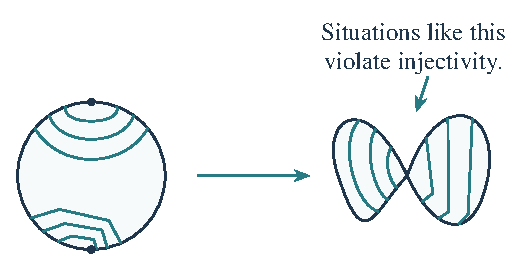
\includegraphics[width=11.5cm]{ms-fig-02.pdf}
\FigureTag{MS2}{fig:ms-02}
\end{figure}

More generally, take $C\subseteq J(f)$ with $f(C)\subseteq C$, and
consider $f\colon\widehat{\mathbb C}\setminus f^{-1}(C)
\to\widehat{\mathbb C}\setminus C$.

\begin{figure}[H]\centering
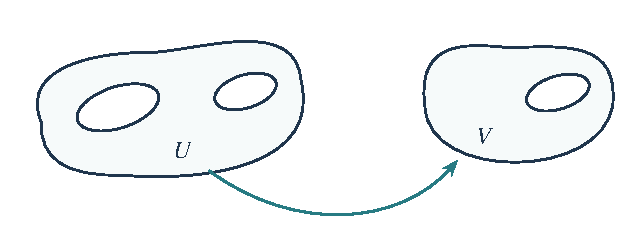
\includegraphics[width=12cm]{ms-fig-04.pdf}
\FigureTag{MS4}{fig:ms-04}
\end{figure}

Here
\[
 \mathcal I(C):=\bigcup_{\substack{V\subseteq\widehat{\mathbb C}\setminus C\\
                         V\text{ a component}}}\mathcal I(V).
\]

\subsection{Regularity of the map}

We loosen the regularity of $f$ for convenience. Sullivan's
straightening theorem says that $f$ is quasirational if and only if
$\langle f^{\circ n}\rangle_n$ is uniformly $K$-quasiregular. Here
quasirational means $f\equiv\varphi\circ R\circ\varphi^{-1}$, with
$R$ rational.

\section{McMullen's gluing lemma}

\paragraph{Hypotheses.}
\begin{enumerate}[label=(\roman*)]
\setcounter{enumi}{0}\item $\mathcal I(U)$ is either a fixed component of $\mathcal I(C)$,
or strictly preperiodic, with $f^{\circ n}(V)\cap U=\varnothing$.
\setcounter{enumi}{1}\item There are quasiconformal maps $\phi_{U,V}\colon U,V\to\mathbb D$
such that $B$ and $f$ are compatible in the following diagram.
\end{enumerate}

\begin{figure}[H]\centering
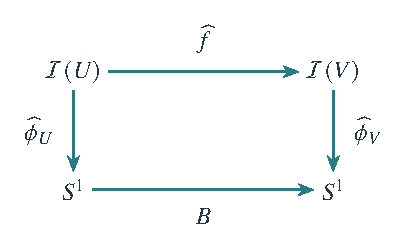
\includegraphics[width=7cm]{ms-fig-06.pdf}
\FigureTag{MS6}{fig:ms-06}
\end{figure}

\begin{claim}
The map
\[
 g(z):=\begin{cases}
 f(z),&z\notin U,\\
 \phi_V^{-1}\circ B\circ\phi_U(z),&z\in U
 \end{cases}
\]
is quasirational.
\end{claim}

The same story holds when $\mathcal I(U)$ is periodic.

\begin{figure}[H]\centering
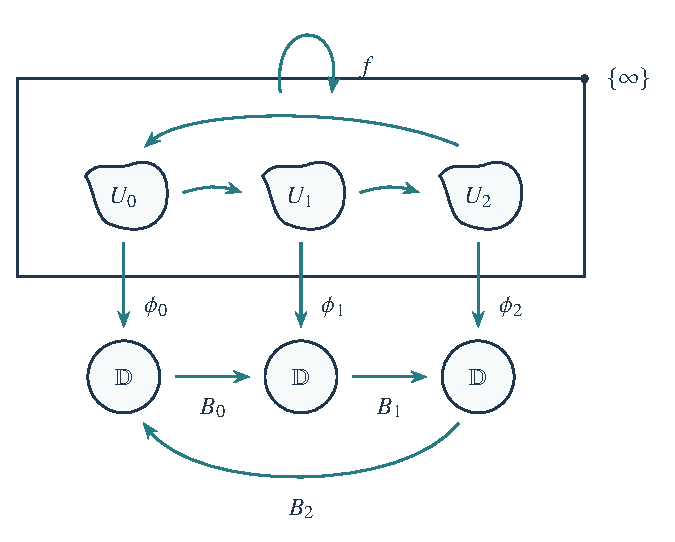
\includegraphics[width=11.5cm]{ms-fig-14.pdf}
\FigureTag{MS14}{fig:ms-14}
\end{figure}

\section{Rigid models}

\begin{enumerate}[label=(\roman*)]
\setcounter{enumi}{0}\item Elliptic: $z\mapsto e^{2\pi i\theta}z$, where
$\theta\in\mathbb R\setminus\mathbb Q$.
\setcounter{enumi}{1}\item Hyperbolic: $z\mapsto z^d$, where $d>1$.
\setcounter{enumi}{2}\item Parabolic: $z\mapsto\dfrac{z^d+a}{1+az^d}$, where
$a=\dfrac{d-1}{d+1}$.
\end{enumerate}

\paragraph{Goal.}
Simplify rational maps by gluing these rigid models along $\mathcal I(C)$
for $C\subseteq J(R)$.

\section{Application of McMullen's surgery}

\setcounter{theorem}{1}\begin{theorem}\label{thm:application}
Let $C\subseteq J(f)$ be a forward-invariant, closed component.
Then $f|_C\sim g|_{J(g)}$, where $g$ is built out of rigid models.
\end{theorem}

\subsection{Dynamics on the ideal boundary}

Only finitely many components $V_1,\ldots,V_k$ of
$\widehat{\mathbb C}\setminus C$ intersect $f^{-1}(C)$ or contain
a critical point. Denote this collection by $\mathcal V$.

\begin{enumerate}[label=(\roman*)]
\setcounter{enumi}{0}\item If $U\notin\mathcal V$ is a component of
$\widehat{\mathbb C}\setminus C$, then
$f|_U\colon U\to f(U)$ is a covering. Since $U$ is a disc,
$\deg(f)=1$. Thus $\deg(f)>1$ on only finitely many components of
$\widehat{\mathbb C}\setminus C$.

\end{enumerate}

\subsection{Periodic components and the surgery}

\setcounter{theorem}{2}\begin{lemma}\label{lem:periodic-compatibility}
On periodic components of $\mathcal I(C)$, the first return map is
compatible with one of the rigid models.
\end{lemma}
% BLOG-CONTENT-END
\end{document}
